\chapter{Bewertung} \chaplabel{bewertung}

In diesem Kapitel bewerte ich den nach unserem Design umgesetzten
Datenhandschuh und das Gesamtsystem. Ich gehe dabei auf die Datenqualität ein,
und stelle Probleme vor, die diese negativ beeinflusst haben. Danach bewerte
ich, ob wir unsere Designziele aus \chapref{ziele} erreicht haben, und erwähne
mögliche Verbesserungen, die wir am System noch erkannt haben.

\section{Datenqualität} \seclabel{datenqualitaet}

Die vom Handschuh ermittelten Daten sind von ausreichender Qualität, wenn man
an ihnen unterschiedliche Tastenanschläge erkennen kann. Nur dann ist auch ein
ML-Al\-go\-rith\-mus in der Lage, diese Erkennung ebenfalls durchzuführen.

\begin{figure}
    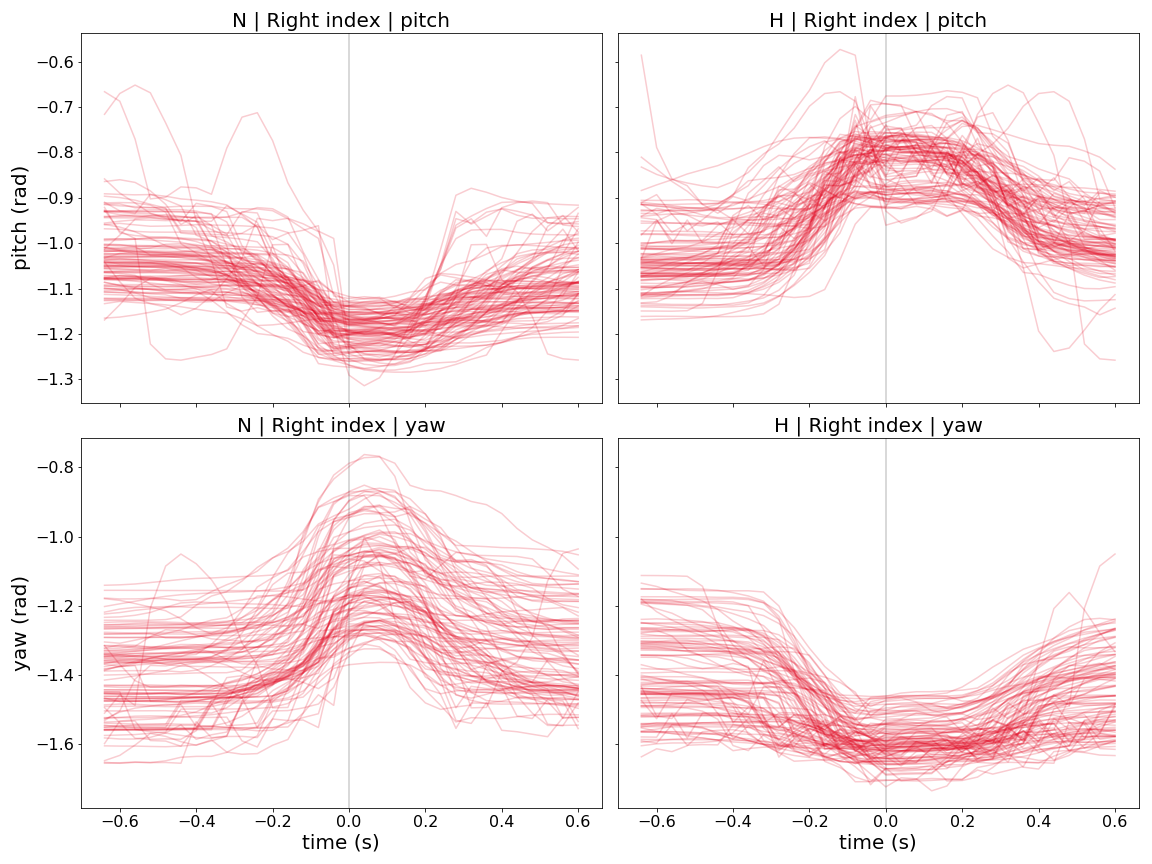
\includegraphics[width=\textwidth]{../common/images/plot-samples-2x2}
    \caption[Einzelne Samples der Tastendrücke N und H]{Mehrere Wiederholungen
    der Tasten N und H, überlagert zum Zeitpunkt des Drückens der Taste
    (Mittellinie). Gezeichnet sind zur einfacheren Visualiserung der relative
    Pitch"~ und Yaw-Winkel des rechten Zeigefingers. Der Zeigefinger liegt
    zwischen den Tastendrücken in Ruheposition auf der Taste H.}
    \figlabel{plot-samples-2x2}
\end{figure}

\figref{plot-samples-2x2} zeigt die extrahierten, vorverarbeiteten Daten aus
Phase 1. Auf der linken Seite wurde die Taste \keyboard{N} und auf der rechen
Seite die Taste \keyboard{H} gedrückt. In den oberen Graphen ist der
Pitch-Winkel, unten der Yaw-Winkel des rechten Zeigefingers relativ zur
Handbasis aufgezeichnet.  Entlang der x-Achse ist die Zeit vor und nach dem
Tastenanschlag aufgeführt, zum Zeitpunkt des Tastenanschlages ist eine
Hilfslinie im Graphen eingezeichnet.  Jedes Sample (also jeder Tastendruck)
tritt als einzelne Linie im Graphen auf. Anhand diesen Samples wird das Netz
trainiert\footnote{Tatsächlich benutzen wir für das Training die Quaternionen,
wir zeigen hier die Euler-Winkel, da diese einfacher zu verstehen sind.}.

Die Unterschiede in den Bewegungsmustern für die verschiedenen Tastenanschläge
sind hier gut zu erkennen. Wir stellen fest, dass sich alle Samples innerhalb
des gleichen Graphen bis auf einige Ausnahmen sehr ähneln -- dies ist wichtig
für die Erkennung eines Musters.  Die Amplitude des Ausschlages ist jeweils
vergleichbar, einzig der y-Offset ist teilweise von Sample zu Sample
unterschiedlich (gut erkennbar im N-Yaw-Graphen).

\begin{figure}[p]
    \centering
    \advance\leftskip-2cm
    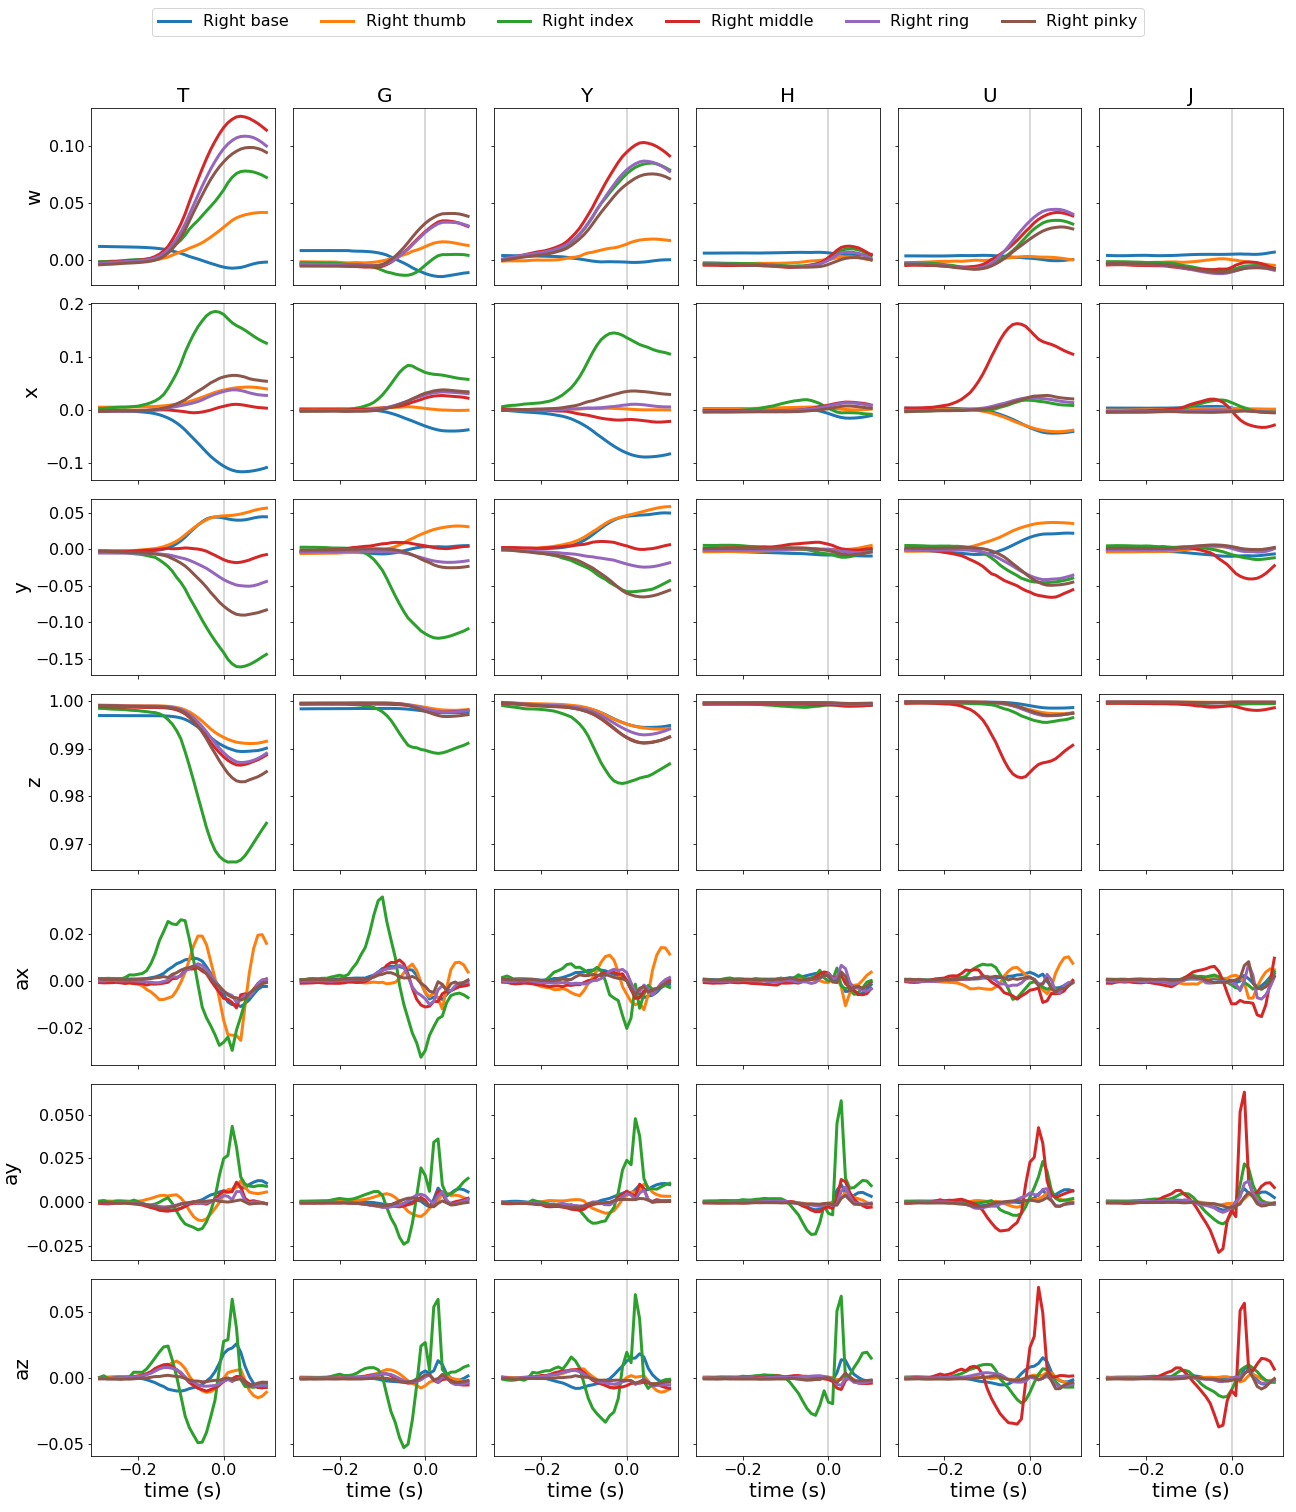
\includegraphics[width=17cm]{../common/images/graphs-average}
    \caption[Mittel aller Samples verschiedener Tastenanschläge aus
    Phase~2]{Mittel aller Samples verschiedener Tastenanschläge aus Phase~2,
    aufgeteilt nach Eingabewert und Sensor. Auf der x-Achse ist die Zeit vor
    und nach dem Tastenanschlag aufgetragen, die y-Achse zeigt den jeweiligen
    Eingabewert (v.o.n.u Quaternion w, x, y, z, Accelerometer x, y, z in
    $m/s^2$).  Für jede Taste wurden etwa 150 Samples aufgezeichnet.}
    \figlabel{graphs-average}
\end{figure}

\figref{graphs-average} enthält viele verschiedene Graphen, welche aus den
Aufzeichnungen für Phase 2 (siehe \chapref{ml}) extrahiert wurden. Für einen
Teil der Tasten\footnote{Phase 2 enthält 10 verschiedene Tasten, wir zeigen zur
Übersicht nur 6 davon.} werden hier sowohl die Quaternionen, als auch die
Accelerometerdaten über die Zeit aufgezeichnet. Der Tastenanschlag liegt nun
bei drei Vierteln des gezeichneten Zeitfensters. Jeder Subgraph enthält 6
Kurven, jeweils eine für jeden der Sensoren der rechten Hand. Die einzelne
Kurve ist dabei das Mittel aller für diesen Sensor, Tastenanschlag und
Eingabewert ermittelten Samples.

Für jede der gezeigten Tasten ist in diesen Graphen ein eindeutiges Muster
erkennbar. Beispielsweise sind sich die Muster der Tasten \keyboard{T} und
\keyboard{Y} sehr ähnlich, unterscheiden sich jedoch im Ausschlag der
z-Komponente der Quaternion des rechten Zeigefingers. Dass sich die Muster für
diese Tasten grundsätzlich ähnlich sind, ist verständlich, da sie direkt
benachbart sind, und der Zeigefinger für beide Tasten eine Bewegung nach oben
links von der Ruheposition aus machen muss.

Ein anders Beispiel sind die Tasten \keyboard{H} und \keyboard{J}. Diese
unterscheiden sich auf den ersten Blick nur geringfügig im Muster, es wird fast
keine Änderung an der Orientierung der Sensoren festgestellt. Das liegt daran,
dass in Ruheposition des Probanden der Zeige- und Mittelfinger auf diesen
Tasten liegen, und somit kaum eine Bewegung durchgeführt werden muss. Bei
genauerer Betrachtung stellt man jedoch fest, dass der y- und z-Ausschlag des
Accelerometers von verschiedenen Sensoren stammt, das \keyboard{H} wird also
eindeutig mit dem Zeigefinger betätigt und das \keyboard{J} mit dem
Mittelfinger.

Wir sind grundsätzlich mit der Qualität dieser Daten sehr zufrieden und halten
sie für geeignet, um damit eine Klassifizierung durchzuführen. Zu beachten ist
aber, dass diese Daten schon vorverarbeitet worden sind. Einige der
nachfolgend genannten Probleme wurden in der Vorverarbeitung dabei bereits
behoben.

Es handelt sich bei den gezeigten um im Laborversuch gewonnene Daten. Reale
Daten werden sicher noch ungenauer und uneindeutiger, wir hoffen hier mit
weiteren Verbesserungen der Vorverarbeitungsmethoden gegensteuern zu können und
mehr Eindeutigkeit zu erreichen.

\section{Probleme} \seclabel{probleme}

Im folgenden zeige ich die Probleme auf, welche wir im Laufe unserer Arbeit festgestellt
haben.

\subsection{Gyro clipping}

Im Fusionsmodus, den wir für die Berechnung der Quaternionen aktiviert haben,
steuert die BNO intern die Sensorkonfiguration, sodass sich diese nicht mehr
von außen festlegen lässt, wie es etwa im Rohdaten-Modus der Fall wäre.
Außerdem übernimmt der Fusionsalgorithmus die Kontrolle über die initiale
Kalibrierung der Sensoren und führt Selbsttests und Echtzeitkalibrierungen
durch.

Leider können wir einige Probleme mit dem Fusionsalgorithmus der BNO055
feststellen\footnote{Im Adafruit Forum gibt es eine lange Diskussion zu
verschiedenen Problemen, die andere Benutzer mit der BNO055 erfahren haben,
darunter auch die hier beschriebenen.
\url{https://forums.adafruit.com/viewtopic.php?f=19&t=78459}}. So ist das
Gyroskop fest auf einen Wertebereich von $\SI{\pm500}{deg/s}$ eingestellt, man
kann hierauf keinen Einfluss nehmen. Dreht man den Sensor schneller als dieses
Limit, wird der Wert abgeschnitten, und die Integration der Geschwindigkeit
liefert eine falsche Orientierung. Diese schnellen Bewegungen treten bei
flüssigem Tippen auf.

Wir konnten dies nachstellen, indem wir den Sensor senkrecht platzierten und
von dort schnell in die Waagerechte drehten. Die berechnete Quaternion kommt
dann nicht ganz der Drehung hinterher, es beinhaltet dann Fehler in der Pitch-
und Roll-Komponente.

Eine mögliche Lösung hierfür wird zusammen mit dem folgenden Problem im
nächsten Abschnitt diskutiert.

\subsection{Heading drift}

Ein weiteres Problem ist eine Ungenauigkeit des Headings, also der horizontalen
Ausrichtung. Nach ruckartigen Bewegungen in nicht-waagerechter Orientierung
verliert der Sensor seine Ausrichtung nach Norden. Wir vermuten, dass dies an
der Konfiguration des Kalman-Filters liegt\footnote{Es ist nicht im Datenblatt
der BNO055 spezifiziert, dass es sich bei dem Fusionsalgorithmus um einen
Kalman-Filter handelt, Benutzer ,,Richart100'' im ,,Chief Delphi''-Forum legt
diese Vermutung jedoch nahe: ,,The on-board fusion algorithm, although
unspecified, is likely a Kalman filter variant.''
(\url{https://www.chiefdelphi.com/forums/showthread.php?t=141100}, entnommen am
31.05.2017)}. Dieser bewertet die Genauigkeit des Gyroskopes höher als die des
Magnetometers, vermutlich da das Magnetometer von außen durch Veränderungen im
Magnetfeld beeinflussbar ist. Die Abweichung betrifft nur das Heading, also die
Komponente, die nicht durch den vom Accelerometer gemessenen Gravitationsvektor
korrigiert werden kann.

Diese Abweichung in der Ausrichtung bleibt auch über längere Zeit bestehen,
selbst bei Bewegung des Sensors. Dies erschwert lange Aufzeichnungen mit dem
Handschuh, da die gemessenen Quaternionen zwischendurch ,,verrutschen'' können
und die Samples uneindeutig werden.

Um die Probleme mit dem Gyroskop und dem Drift zu lösen, probieren wir den
Fusionsalgorithmus von \citet{madgwick} aus. Hierfür betreiben wir die BNO055
im Fusionsmodus, lesen aber auch die Rohdaten von Accelerometer, Gyroskop und
Magnetometer aus. Die Rohdaten lassen wir vom Madgwick-Algorithmus in eine
Orientierung umwandeln und vergleichen diese mit der Ausgabe des internen
Fusionsalgorithmus, indem wir beide zu Euler-Winkeln konvertieren und über die
Zeit zeichnen. Die Konvertierung in Euler-Winkel ermöglicht es uns, zwischen
der horizontalen und vertikalen Ausrichtung zu unterscheiden.

Das Ergebnis ist in \figref{madgwick} zu sehen. Wir erkennen, dass die
Algorithmen grundsätzlich sehr ähnliche Ergebnisse liefern.

\begin{figure}
    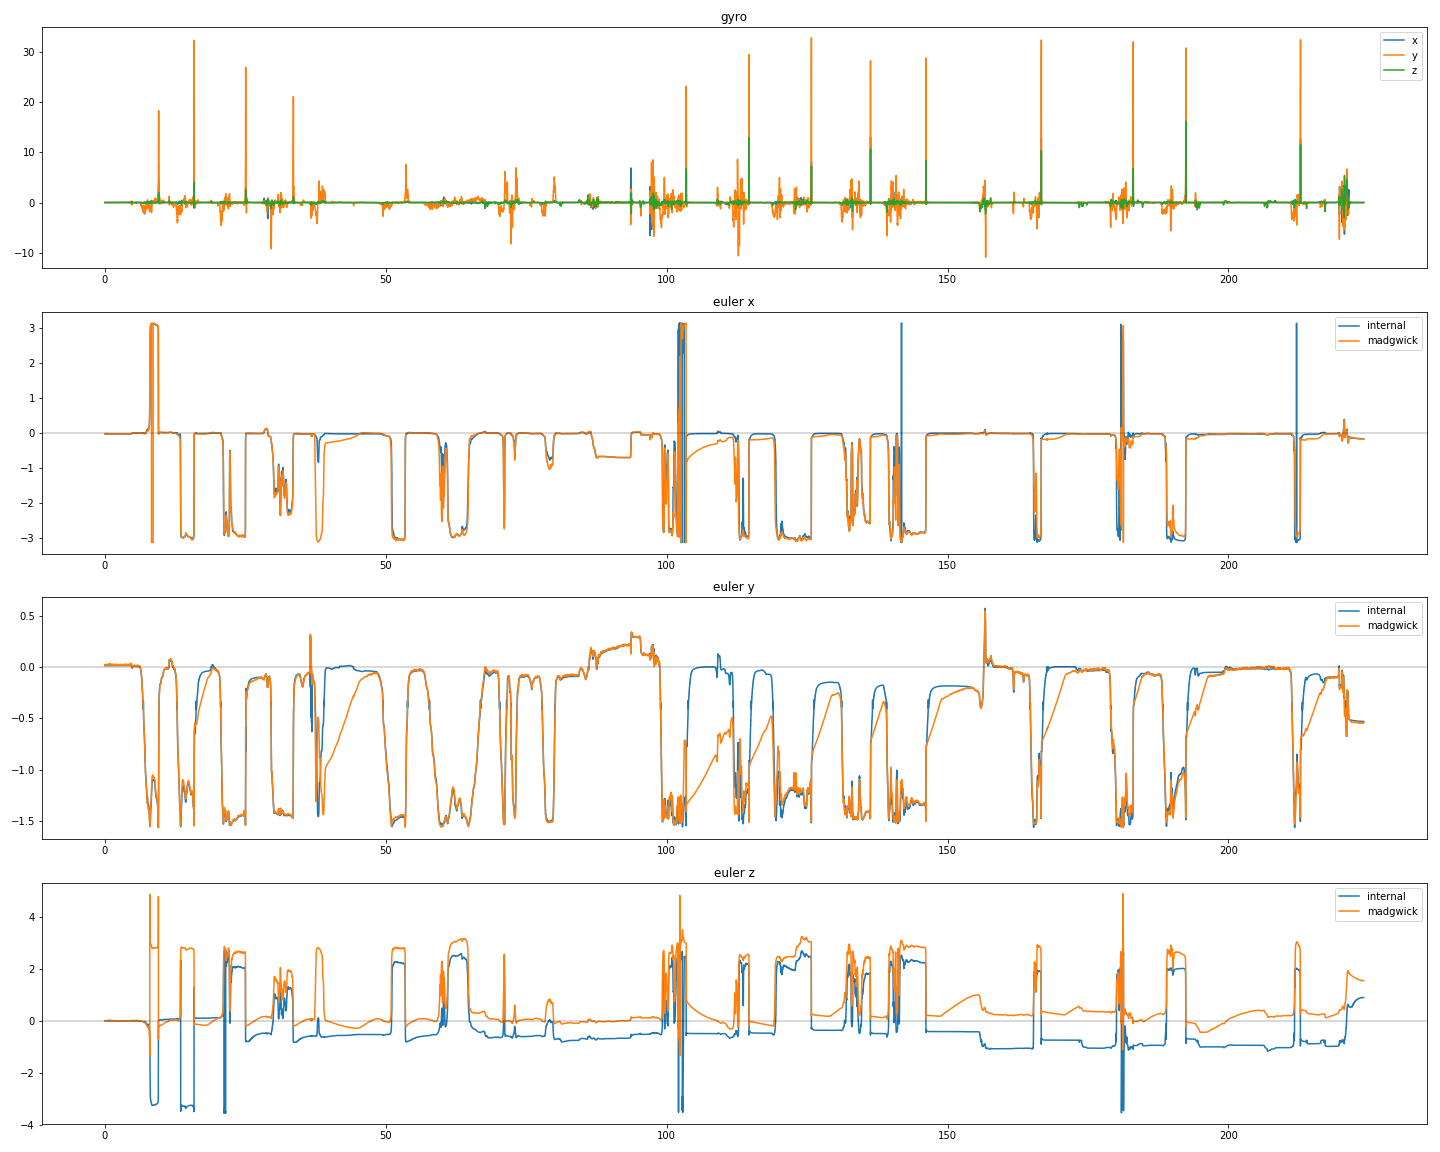
\includegraphics[width=\textwidth]{../data/heading/heading}
    \caption[Interner Fusionsalgorithmus der BNO055 und Madgwick-Algorithmus im
    Vergleich]{Interner Fusionsalgorithmus der BNO055 und Madgwick-Algorithmus
    im Vergleich. Gezeigt sind Rohdaten des Gyroskops (in
    \si{\radian\per\second}) sowie Euler-Winkel der
    Orientierung (in \si{\radian}).}
    \figlabel{madgwick}
\end{figure}

Im unteren Graphen sehen wir, dass die horizontale Ausrichtung nach den
Bewegungsphasen beim Madgwick-Algorithmus (orange) sich immer wieder dem
Initialwert annähert. Der interne Algorithmus weist hier stattdessen den
beschriebenen Drift auf -- nach 200 Sekunden ist das Heading um knapp
\SI{1}{\radian} zu niedrig, und korrigiert sich nicht wieder.

Der Madgwick-Algorithmus konvergiert jedoch viel langsamer zur korrekten
vertikalen Orientierung, wenn er aufgrund schneller Rotation eine Differenz
zwischen Gravitationsrichtung und gemessener Ausrichtung erkennt.  Dies lässt
sich besonders gut im dritten Graphen erkennen. Teilweise dauert es bis zu 10
Sekunden, bis sich der Wert an den des internen Algorithmus annähert.

Diese Konvergenz lässt sich durch Anpassung des ,,Gain''-Parameters
beschleunigen, jedoch rät Madgwick davon ab, da es das Rauschen verstärkt.  Das
konnten wir leicht überprüfen, die Ausrichtung fängt mit höherem Gain-Wert an
zu zittern. Dies ließe sich eventuell korrigieren, indem man den Wertebereich
der Sensoren erhöht, und somit die Sensitivität verringert. Allerdings müssten
wir dafür den Fusionsmodus deaktivieren und würden die automatische
Echtzeit-Selbstkalibrierung des Sensors verlieren.

% \begin{itemize}
%     \item gyro clippt bei 500 deg/s
%     \item aus senkrechter zurück in waagerechte ist schwer
%     \item Problem:
%     \item es gibt einen alternative algorithmus von Madgwick
%     \item der soll das angeblich können
% \end{itemize}
%

\subsection{Robustheit}

Unser Prototyp erwies sich nicht als besonders langlebig. Nach einigen
Experimenten brachen teilweise die Lötstellen auf, da sie durch die
Handbewegungen vielen Biegungszyklen ausgesetzt waren. Dies ist jedoch
lediglich ein Problem des Prototyps, und keine allgemeine Einschränkung. Einige
Zugentlastungen, eine einteilige Bauweise ohne Steckverbindungen,
eingeschweißte Sensoren sowie mehradrige Kabelverbindungen würden die
Robustheit des Handschuhs deutlich erhöhen.

\subsection{Verwendung einer Laptop-Tastatur}

In unseren Versuchen haben wir die in einen Laptop eingebaute Tastatur
verwendet, welche im Vergleich zu Standard-Tastaturen relativ flach ist.
Dadurch ist die Änderung der Orientierung für einige Tasten sehr gering, es
handelt sich dabei um jene Tasten, auf denen die Finger in Ruheposition liegen
(\keyboard{H}, \keyboard{J}, \keyboard{\spacebar}). Der Algorithmus hat es
dementsprechend schwer, diese Tasten richtig zu klassifizieren, und verwechselt
sie ebenfalls mit der Klasse $\emptyset$. Erst in einer Wiederholung des
Experiments lernte der Algorithmus, diese Tasten zu unterschieden werden,
jedoch mit wesentlich geringerer Genauigkeit als die anderen Tasten. Vermutlich
liegt dieses andere Ergebnis an einer zufällig besseren Initialisierung der
Parameter im Netz.

Die Verwendung einer Tastatur mit genügend Tastenhub würde sicherlich
bessere Ergebnisse erzielen. Außerdem erkennt man, wie in
\figref{graphs-average} gesehen, an den Beschleunigungsdaten Unterschiede. Es
wäre daher ebenfalls gut, den Klassifikator anzupassen, sodass er ebenfalls
die Rohdaten des Accelerometers verwendet.

\section{Sekundäre Designziele}

In diesem Abschnitt gehe ich auf die im \chapref{ziele} vorgestellten Ziele ein
und bewerte, inwieweit wir diese Ziele erfüllt haben. Das primäre Designziel,
charakteristische Werte zu extrahieren, haben wir bereits in
\secref{datenqualitaet} bewertet, und festgestellt, dass die Auswahl und
Qualität der Daten unseren Anforderungen entsprechen.

\subsection{Performance}

\begin{figure}
    \centering
    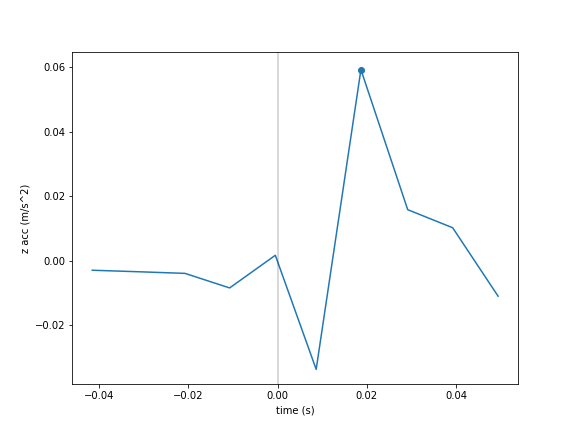
\includegraphics[width=10cm]{../common/images/delay}
    \caption[Messung der Verzögerung der IMU-Daten]{Messung der Verzögerung der IMU-Daten anhand der z-Komponente der
    Beschleunigung. Die IMU wird zusammen mit der Taste heruntergedrückt. Der
    dazugehörige Ausschlag des Accelerometers wird erst einige Zeit (hier
    \SI{18.6}{\milli\second}) nach dem Tastendruck (Zeitpunkt 0) registriert.
    Im Schnitt ergibt sich eine Verzögerung von rund \SI{15}{\milli\second}.}
    \figlabel{performance}
\end{figure}

Bezüglich der Performance haben wir unser Ziel, die angestrebte Datenrate von
\SI{100}{Hz}, fast erreicht. In unserem Messungen ermittelten wir eine
durchschnittliche Datenrate von rund \SI{90}{Hz}.

Die Verzögerung in der Datenübertragung von den Sensoren bis zum Host-PC ist
ist relativ gering.  In einem Experiment hierzu legten wir eine IMU auf die
Tastatur und drückten sie zusammen mit der Taste herunter.  Das Ergebnis dieses
Experiments ist in \figref{performance} zu sehen. Innerhalb von
durchschnittlich \SI{15}{ms} nach dem Tastenanschlag war der Ausschlag am
Accelerometer sichtbar. Hiervon sind bis zu \SI{10}{ms} durch die Datenrate
bedingt, die restliche Verzögerung kommt durch die Übertragung zustande.

\subsection{Geringe motorische Einschränkung}

Der Handschuh schränkt beim Tippen kaum ein. Die Finger sind größtenteils frei
beweglich. Man kann die Hand zur Faust formen, oder die Finger weit spreizen.

Bringt man die Finger dicht zusammen, reiben die Gummibänder an den
Nachbarfingern. Dies ist jedoch beim Tippen nicht nötig, weil die Tasten einer
Standard-Tastatur weiter auseinander liegen als die Finger breit sind. Auch im
Alltag ist ein Zusammenbringen der Finger eine eher unnatürliche Haltung, daher
werten wir diesen Nachteil als nicht besonders wichtig.

Der Handschuh ist leicht (ca. \SI{70}{g} mit Akku), sodass die Hand auch bei
längerer Benutzung nicht ermüdet. Weil der Handschuh aus einfachem, dünnem
Baumwollstoff gefertigt ist, schwitzt man auch nicht darin. Die Gummiringe
schränken die Durchblutung der Finger nicht ein, sitzen aber fest genug auf dem
Finger.  Hierfür ist es natürlich wichtig, dass die Fingerringe auf den
Fingerumfang des Benutzers angepasst sind.

Der Handschuh ist alltagstauglich, übliche Büroaktivitäten zum Beispiel lassen
sich mit Handschuh uneingeschränkt durchführen. Getestet wurden zum Beispiel
das Öffnen von Türen, Greifen und Verwenden einer Kaffeetasse und die Benutzung
von Stiften. Etwas weniger geeignet ist der Handschuh bei sehr feinmotorischer
Interaktion mit Gegenständen, etwa wenn man einen Reißverschluss schließen
möchte -- dies liegt jedoch daran, dass der Prototyp nicht besonders robust
ist. Dank der freiliegenden Fingerkuppen sind feine Manipulationen dieser Art
trotzdem möglich.

\subsection{Haltungsunabhängigkeit}

Dieses Ziel haben wir bisher nur in beschränktem Maße erreicht. Prinzipiell ist
die Benutzung in verschiedenen Ausrichtungen möglich, da die relative
Orientierung der Sensoren ermittelt wird. Allerdings ist die BNO055 in der
Senkrechten nicht so genau wie in der Waagerechten, vermutlich liegt das am
internen Fusionsalgorithmus. Die ermittelte Orientierung springt hierbei
teilweise um einige Grad.

Dennoch war es uns möglich, mit den Händen in der Luft oder auf dem Tisch zu
tippen. Löst man also das Problem mit den Sensoren, erfüllt das Systemdesign
diese Anforderung.

\subsection{Prototyping-geeignete Software}

Unser Softwaredesign ist sehr gut geeignet, um damit einen Prototyp zu
entwickeln. Dank der flexiblen Konfiguration können wir ohne bedeutenden
Aufwand alle wichtigen Parameter ändern. Auch grundlegendere Aspekte, wie den
verwendeten Typ von neuronalem Netzwerk, stellen wir in der Konfigurationsdatei
ein. Dadurch bleibt jedes Experiment nachvollziehbar und wiederholbar. Dies ist
sehr wichtig, insbesondere wenn das gleiche Experiment mit anderen Daten
wiederholen möchte oder Bugs behoben hat.

Die Verwendung von ROS war ebenfalls eine gute Entscheidung. ROS-Bags sind eine
sehr einfache Methode, Zeitreihen aufzuzeichnen und wieder abzuspielen oder
direkt auszulesen. Mit dem Topic-System bietet ROS darüber hinaus eine flexible
Möglichkeit, Schnittstellen zwischen Programmen zu definieren und einzelne
Verarbeitungsschritte unabhängig zu implementieren. Unabdingbar bei der
Entwicklung eines solchen Systems ist die Möglichkeit, die erfassten und
verarbeiteten Daten zur Fehlerbehebung zu visualisieren -- ROS und die
ROS-Community liefern hierfür zahlreiche Programme.

\subsection{Ausbaufähigkeit zu marktfähigem Produkt}

Der Prototyp ist, wie bereits bemerkt, nicht sonderlich robust. Ein industriell
gefertigtes Produkt könnte diese Schwächen doch in unseren Augen gut
überwinden, mit entsprechendem Aufwand wäre eine hochwertige Produktion sicher
möglich. Durch die Verwendung von IMUs als Sensoren haben wir hierzu die
Grundlage geschaffen, da IMUs in sich abgeschlossen und robust sind und ohne
bewegliche Teile auskommen.

Die Bauteile für den Prototyp waren in der Anschaffung sehr teuer. Die
Sensoren mit jeweils \EUR{24,00} machen hierbei einen Großteil der Kosten aus,
insgesamt kommen wir auf etwa \EUR{200}. In industrieller Massenproduktion wäre
man nicht auf die Verwendung von verfügbaren Breakout-Boards angewiesen und
könnte die Bauteile selbst vom Hersteller beziehen und auf einer speziell
gefertige Leiterplatte anbringen. Wir haben die Kosten für den Prototyp und
das Endprodukt geschätzt und in \tabref{kosten} aufgeführt.  Demnach könnte ein
,,consumer ready'' Handschuh pro Stück unter \EUR{100}, bzw. \EUR{200} für eine
komplette ,,Tastatur'', kosten. Eine hochwertige ergonomische Tastatur liegt
heutzutage bei einem vergleichbaren Preis.

Dass man mit diesem Hardwareaufbau ein marktfähiges Produkt herstellen kann,
zeigt auch der Hi5 VR Glove~\cite{web:hi5vrglove}.

\begin{table}
    \centering
    \renewcommand{\arraystretch}{1.2}
    \begin{tabular}{@{}llrr@{}}
        \toprule
        & \phantom{X} & \multicolumn{2}{c}{Kosten in \euro} \\
        \cmidrule{3-4}
        Komponente & & Prototyp & Produktion \\
        \midrule
        IMUs & & $6\times24.00$ & $6\times7.00$ \\
        Mikroprozessor (Cortex M0) & & $42.00$ & $2.60$ \\
        WLAN-Modul (ATWINC1500) & & $\ast$ & $5.00$ \\
        Sekundärbauteile (Widerstände etc.) & & $\ast$ & $10.00$ \\
        Akku & & $5.00$ & $5.00$ \\
        Leiterplatte & & \textendash{} & $10.00$ \\
        Verkabelung, Steckverbindungen & & $10.00$ & $10.00$ \\
        Handschuh & & $0.20$ & $5.00$ \\
        \midrule
        \textbf{Summe} & & $201.20$ & $84.60$ \\
        \bottomrule
    \end{tabular}
    \\[1.5ex]
    $\ast$ bereits im Mikroprozessor enthalten
    \caption[Kostenübersicht für die Herstellung eines
    Handschuhs]{Kostenübersicht für die Herstellung eines Handschuhs. Preise für
    IC-Bausteine wurden ermittelt von \url{http://www.mouser.de/} am 26. Mai
2017, restliche Kosten sind Schätzwerte.}
    \tablabel{kosten}
\end{table}

\section{Verbesserungsmöglichkeiten}

Für die Zukunft sehe ich noch einigen Raum für Verbesserungen am Design und der
Umsetzung des Systems.

Selbstverständlich wäre es gut, die Probleme bei der Datenerfassung zu beheben.
Evaluieren könnte man dafür andere IMUs, welche jeweils mit ihrem proprietären
Fusionsalgorithmus ausgeliefert werden. Zusätzlich wäre es interessant, die
BNO055 selbst zu kalibrieren, an der Konfiguration der Sensoren zu
experimentieren, und dann einen verfügbaren Fusionsalgorithmus, zum Beispiel
von \citet{madgwick}, oder einen Kalman-Filter auszuprobieren.  Anstatt dieses
Problem in der Datenerfassung zu lösen, wäre es ebenfalls denkbar, eine
geeignete Fehlererkennung in der Vorverarbeitung zu implementieren und die
Messwerte anhand des ermittelten Fehlers anzupassen.  Hier besteht großes
Optimierungspotenzial, sicherlich wäre es mit einigem Aufwand möglich,
wesentlich genauere Daten ohne Clipping oder Drift zu erhalten. Die Evaluation
dieser Lösungsansätze ist jedoch aufgrund des hohen Aufwandes nicht Teil unsere
Bachelorarbeiten.

Der Handschuh an sich ließe sich robuster gestalten, auch in Form eines
Prototyps. Für einen hochwertigerer Handschuh könnte man die Finger-Ringe mit
dem Handschuh zu verbinden, und eventuell auch das am Handgelenk befestigte
Teil in den Handschuh integrieren. Damit wäre der Handschuh einteilig und hätte
weniger anfällige Verbindungsstellen.

Das System unterstützt bisher nur den Betrieb entweder über USB, oder über
WLAN. Diese Konfiguration muss fest in der Firmware hinterlegt werden, ein
Umschalten im Live-Betrieb ist dadurch nicht möglich. Diese Funktionalität,
sowie eine Verbesserung der Robustheit der Übertragung (eine
Übertragungsunterbrechung erfordert zurzeit einen Neustart des Prozessors)
könnten in der Zukunft implementiert werden. Besonders interessant wird dies,
wenn man hauptsächlich den WLAN-Modus verwendet, und die Verbindung bei
Bewegung im Gebäude unterbrochen wird.

Natürlich sind ebenfalls Verbesserungen am Lernalgorithmus vonnöten, um ein
konkurrenzfähiges Produkt zu erschaffen. Weitere Forschung wird die angestrebte
Zuverlässigkeit und Genauigkeit erhöhen. Einige Ideen und Ansätze hierfür
werden in der Arbeit von Carolin \citet{caro} aufgezeigt.

Außerdem wäre es schön, ein einfaches Benutzerinterface zur Konfiguration des
Handschuhs und zum Training des ML-Algorithmus zu entwickeln. Hiermit könnte
man die WLAN-Zugangsdaten festlegen und Profile für verschiedene Benutzer oder
Anwendungen verwalten.

% vim: tw=79
